
\documentclass[10pt]{article} % For LaTeX2e
% \usepackage{tmlr}
% If accepted, instead use the following line for the camera-ready submission:
%\usepackage[accepted]{tmlr}
% To de-anonymize and remove mentions to TMLR (for example for posting to preprint servers), instead use the following:
\usepackage[preprint]{tmlr}
\usepackage{graphicx}
% Optional math commands from https://github.com/goodfeli/dlbook_notation.
%%%%% NEW MATH DEFINITIONS %%%%%

\usepackage{amsmath,amsfonts,bm}

% Mark sections of captions for referring to divisions of figures
\newcommand{\figleft}{{\em (Left)}}
\newcommand{\figcenter}{{\em (Center)}}
\newcommand{\figright}{{\em (Right)}}
\newcommand{\figtop}{{\em (Top)}}
\newcommand{\figbottom}{{\em (Bottom)}}
\newcommand{\captiona}{{\em (a)}}
\newcommand{\captionb}{{\em (b)}}
\newcommand{\captionc}{{\em (c)}}
\newcommand{\captiond}{{\em (d)}}

% Highlight a newly defined term
\newcommand{\newterm}[1]{{\bf #1}}


% Figure reference, lower-case.
\def\figref#1{figure~\ref{#1}}
% Figure reference, capital. For start of sentence
\def\Figref#1{Figure~\ref{#1}}
\def\twofigref#1#2{figures \ref{#1} and \ref{#2}}
\def\quadfigref#1#2#3#4{figures \ref{#1}, \ref{#2}, \ref{#3} and \ref{#4}}
% Section reference, lower-case.
\def\secref#1{section~\ref{#1}}
% Section reference, capital.
\def\Secref#1{Section~\ref{#1}}
% Reference to two sections.
\def\twosecrefs#1#2{sections \ref{#1} and \ref{#2}}
% Reference to three sections.
\def\secrefs#1#2#3{sections \ref{#1}, \ref{#2} and \ref{#3}}
% Reference to an equation, lower-case.
\def\eqref#1{equation~\ref{#1}}
% Reference to an equation, upper case
\def\Eqref#1{Equation~\ref{#1}}
% A raw reference to an equation---avoid using if possible
\def\plaineqref#1{\ref{#1}}
% Reference to a chapter, lower-case.
\def\chapref#1{chapter~\ref{#1}}
% Reference to an equation, upper case.
\def\Chapref#1{Chapter~\ref{#1}}
% Reference to a range of chapters
\def\rangechapref#1#2{chapters\ref{#1}--\ref{#2}}
% Reference to an algorithm, lower-case.
\def\algref#1{algorithm~\ref{#1}}
% Reference to an algorithm, upper case.
\def\Algref#1{Algorithm~\ref{#1}}
\def\twoalgref#1#2{algorithms \ref{#1} and \ref{#2}}
\def\Twoalgref#1#2{Algorithms \ref{#1} and \ref{#2}}
% Reference to a part, lower case
\def\partref#1{part~\ref{#1}}
% Reference to a part, upper case
\def\Partref#1{Part~\ref{#1}}
\def\twopartref#1#2{parts \ref{#1} and \ref{#2}}

\def\ceil#1{\lceil #1 \rceil}
\def\floor#1{\lfloor #1 \rfloor}
\def\1{\bm{1}}
\newcommand{\train}{\mathcal{D}}
\newcommand{\valid}{\mathcal{D_{\mathrm{valid}}}}
\newcommand{\test}{\mathcal{D_{\mathrm{test}}}}

\def\eps{{\epsilon}}


% Random variables
\def\reta{{\textnormal{$\eta$}}}
\def\ra{{\textnormal{a}}}
\def\rb{{\textnormal{b}}}
\def\rc{{\textnormal{c}}}
\def\rd{{\textnormal{d}}}
\def\re{{\textnormal{e}}}
\def\rf{{\textnormal{f}}}
\def\rg{{\textnormal{g}}}
\def\rh{{\textnormal{h}}}
\def\ri{{\textnormal{i}}}
\def\rj{{\textnormal{j}}}
\def\rk{{\textnormal{k}}}
\def\rl{{\textnormal{l}}}
% rm is already a command, just don't name any random variables m
\def\rn{{\textnormal{n}}}
\def\ro{{\textnormal{o}}}
\def\rp{{\textnormal{p}}}
\def\rq{{\textnormal{q}}}
\def\rr{{\textnormal{r}}}
\def\rs{{\textnormal{s}}}
\def\rt{{\textnormal{t}}}
\def\ru{{\textnormal{u}}}
\def\rv{{\textnormal{v}}}
\def\rw{{\textnormal{w}}}
\def\rx{{\textnormal{x}}}
\def\ry{{\textnormal{y}}}
\def\rz{{\textnormal{z}}}

% Random vectors
\def\rvepsilon{{\mathbf{\epsilon}}}
\def\rvtheta{{\mathbf{\theta}}}
\def\rva{{\mathbf{a}}}
\def\rvb{{\mathbf{b}}}
\def\rvc{{\mathbf{c}}}
\def\rvd{{\mathbf{d}}}
\def\rve{{\mathbf{e}}}
\def\rvf{{\mathbf{f}}}
\def\rvg{{\mathbf{g}}}
\def\rvh{{\mathbf{h}}}
\def\rvu{{\mathbf{i}}}
\def\rvj{{\mathbf{j}}}
\def\rvk{{\mathbf{k}}}
\def\rvl{{\mathbf{l}}}
\def\rvm{{\mathbf{m}}}
\def\rvn{{\mathbf{n}}}
\def\rvo{{\mathbf{o}}}
\def\rvp{{\mathbf{p}}}
\def\rvq{{\mathbf{q}}}
\def\rvr{{\mathbf{r}}}
\def\rvs{{\mathbf{s}}}
\def\rvt{{\mathbf{t}}}
\def\rvu{{\mathbf{u}}}
\def\rvv{{\mathbf{v}}}
\def\rvw{{\mathbf{w}}}
\def\rvx{{\mathbf{x}}}
\def\rvy{{\mathbf{y}}}
\def\rvz{{\mathbf{z}}}

% Elements of random vectors
\def\erva{{\textnormal{a}}}
\def\ervb{{\textnormal{b}}}
\def\ervc{{\textnormal{c}}}
\def\ervd{{\textnormal{d}}}
\def\erve{{\textnormal{e}}}
\def\ervf{{\textnormal{f}}}
\def\ervg{{\textnormal{g}}}
\def\ervh{{\textnormal{h}}}
\def\ervi{{\textnormal{i}}}
\def\ervj{{\textnormal{j}}}
\def\ervk{{\textnormal{k}}}
\def\ervl{{\textnormal{l}}}
\def\ervm{{\textnormal{m}}}
\def\ervn{{\textnormal{n}}}
\def\ervo{{\textnormal{o}}}
\def\ervp{{\textnormal{p}}}
\def\ervq{{\textnormal{q}}}
\def\ervr{{\textnormal{r}}}
\def\ervs{{\textnormal{s}}}
\def\ervt{{\textnormal{t}}}
\def\ervu{{\textnormal{u}}}
\def\ervv{{\textnormal{v}}}
\def\ervw{{\textnormal{w}}}
\def\ervx{{\textnormal{x}}}
\def\ervy{{\textnormal{y}}}
\def\ervz{{\textnormal{z}}}

% Random matrices
\def\rmA{{\mathbf{A}}}
\def\rmB{{\mathbf{B}}}
\def\rmC{{\mathbf{C}}}
\def\rmD{{\mathbf{D}}}
\def\rmE{{\mathbf{E}}}
\def\rmF{{\mathbf{F}}}
\def\rmG{{\mathbf{G}}}
\def\rmH{{\mathbf{H}}}
\def\rmI{{\mathbf{I}}}
\def\rmJ{{\mathbf{J}}}
\def\rmK{{\mathbf{K}}}
\def\rmL{{\mathbf{L}}}
\def\rmM{{\mathbf{M}}}
\def\rmN{{\mathbf{N}}}
\def\rmO{{\mathbf{O}}}
\def\rmP{{\mathbf{P}}}
\def\rmQ{{\mathbf{Q}}}
\def\rmR{{\mathbf{R}}}
\def\rmS{{\mathbf{S}}}
\def\rmT{{\mathbf{T}}}
\def\rmU{{\mathbf{U}}}
\def\rmV{{\mathbf{V}}}
\def\rmW{{\mathbf{W}}}
\def\rmX{{\mathbf{X}}}
\def\rmY{{\mathbf{Y}}}
\def\rmZ{{\mathbf{Z}}}

% Elements of random matrices
\def\ermA{{\textnormal{A}}}
\def\ermB{{\textnormal{B}}}
\def\ermC{{\textnormal{C}}}
\def\ermD{{\textnormal{D}}}
\def\ermE{{\textnormal{E}}}
\def\ermF{{\textnormal{F}}}
\def\ermG{{\textnormal{G}}}
\def\ermH{{\textnormal{H}}}
\def\ermI{{\textnormal{I}}}
\def\ermJ{{\textnormal{J}}}
\def\ermK{{\textnormal{K}}}
\def\ermL{{\textnormal{L}}}
\def\ermM{{\textnormal{M}}}
\def\ermN{{\textnormal{N}}}
\def\ermO{{\textnormal{O}}}
\def\ermP{{\textnormal{P}}}
\def\ermQ{{\textnormal{Q}}}
\def\ermR{{\textnormal{R}}}
\def\ermS{{\textnormal{S}}}
\def\ermT{{\textnormal{T}}}
\def\ermU{{\textnormal{U}}}
\def\ermV{{\textnormal{V}}}
\def\ermW{{\textnormal{W}}}
\def\ermX{{\textnormal{X}}}
\def\ermY{{\textnormal{Y}}}
\def\ermZ{{\textnormal{Z}}}

% Vectors
\def\vzero{{\bm{0}}}
\def\vone{{\bm{1}}}
\def\vmu{{\bm{\mu}}}
\def\vtheta{{\bm{\theta}}}
\def\va{{\bm{a}}}
\def\vb{{\bm{b}}}
\def\vc{{\bm{c}}}
\def\vd{{\bm{d}}}
\def\ve{{\bm{e}}}
\def\vf{{\bm{f}}}
\def\vg{{\bm{g}}}
\def\vh{{\bm{h}}}
\def\vi{{\bm{i}}}
\def\vj{{\bm{j}}}
\def\vk{{\bm{k}}}
\def\vl{{\bm{l}}}
\def\vm{{\bm{m}}}
\def\vn{{\bm{n}}}
\def\vo{{\bm{o}}}
\def\vp{{\bm{p}}}
\def\vq{{\bm{q}}}
\def\vr{{\bm{r}}}
\def\vs{{\bm{s}}}
\def\vt{{\bm{t}}}
\def\vu{{\bm{u}}}
\def\vv{{\bm{v}}}
\def\vw{{\bm{w}}}
\def\vx{{\bm{x}}}
\def\vy{{\bm{y}}}
\def\vz{{\bm{z}}}

% Elements of vectors
\def\evalpha{{\alpha}}
\def\evbeta{{\beta}}
\def\evepsilon{{\epsilon}}
\def\evlambda{{\lambda}}
\def\evomega{{\omega}}
\def\evmu{{\mu}}
\def\evpsi{{\psi}}
\def\evsigma{{\sigma}}
\def\evtheta{{\theta}}
\def\eva{{a}}
\def\evb{{b}}
\def\evc{{c}}
\def\evd{{d}}
\def\eve{{e}}
\def\evf{{f}}
\def\evg{{g}}
\def\evh{{h}}
\def\evi{{i}}
\def\evj{{j}}
\def\evk{{k}}
\def\evl{{l}}
\def\evm{{m}}
\def\evn{{n}}
\def\evo{{o}}
\def\evp{{p}}
\def\evq{{q}}
\def\evr{{r}}
\def\evs{{s}}
\def\evt{{t}}
\def\evu{{u}}
\def\evv{{v}}
\def\evw{{w}}
\def\evx{{x}}
\def\evy{{y}}
\def\evz{{z}}

% Matrix
\def\mA{{\bm{A}}}
\def\mB{{\bm{B}}}
\def\mC{{\bm{C}}}
\def\mD{{\bm{D}}}
\def\mE{{\bm{E}}}
\def\mF{{\bm{F}}}
\def\mG{{\bm{G}}}
\def\mH{{\bm{H}}}
\def\mI{{\bm{I}}}
\def\mJ{{\bm{J}}}
\def\mK{{\bm{K}}}
\def\mL{{\bm{L}}}
\def\mM{{\bm{M}}}
\def\mN{{\bm{N}}}
\def\mO{{\bm{O}}}
\def\mP{{\bm{P}}}
\def\mQ{{\bm{Q}}}
\def\mR{{\bm{R}}}
\def\mS{{\bm{S}}}
\def\mT{{\bm{T}}}
\def\mU{{\bm{U}}}
\def\mV{{\bm{V}}}
\def\mW{{\bm{W}}}
\def\mX{{\bm{X}}}
\def\mY{{\bm{Y}}}
\def\mZ{{\bm{Z}}}
\def\mBeta{{\bm{\beta}}}
\def\mPhi{{\bm{\Phi}}}
\def\mLambda{{\bm{\Lambda}}}
\def\mSigma{{\bm{\Sigma}}}

% Tensor
\DeclareMathAlphabet{\mathsfit}{\encodingdefault}{\sfdefault}{m}{sl}
\SetMathAlphabet{\mathsfit}{bold}{\encodingdefault}{\sfdefault}{bx}{n}
\newcommand{\tens}[1]{\bm{\mathsfit{#1}}}
\def\tA{{\tens{A}}}
\def\tB{{\tens{B}}}
\def\tC{{\tens{C}}}
\def\tD{{\tens{D}}}
\def\tE{{\tens{E}}}
\def\tF{{\tens{F}}}
\def\tG{{\tens{G}}}
\def\tH{{\tens{H}}}
\def\tI{{\tens{I}}}
\def\tJ{{\tens{J}}}
\def\tK{{\tens{K}}}
\def\tL{{\tens{L}}}
\def\tM{{\tens{M}}}
\def\tN{{\tens{N}}}
\def\tO{{\tens{O}}}
\def\tP{{\tens{P}}}
\def\tQ{{\tens{Q}}}
\def\tR{{\tens{R}}}
\def\tS{{\tens{S}}}
\def\tT{{\tens{T}}}
\def\tU{{\tens{U}}}
\def\tV{{\tens{V}}}
\def\tW{{\tens{W}}}
\def\tX{{\tens{X}}}
\def\tY{{\tens{Y}}}
\def\tZ{{\tens{Z}}}


% Graph
\def\gA{{\mathcal{A}}}
\def\gB{{\mathcal{B}}}
\def\gC{{\mathcal{C}}}
\def\gD{{\mathcal{D}}}
\def\gE{{\mathcal{E}}}
\def\gF{{\mathcal{F}}}
\def\gG{{\mathcal{G}}}
\def\gH{{\mathcal{H}}}
\def\gI{{\mathcal{I}}}
\def\gJ{{\mathcal{J}}}
\def\gK{{\mathcal{K}}}
\def\gL{{\mathcal{L}}}
\def\gM{{\mathcal{M}}}
\def\gN{{\mathcal{N}}}
\def\gO{{\mathcal{O}}}
\def\gP{{\mathcal{P}}}
\def\gQ{{\mathcal{Q}}}
\def\gR{{\mathcal{R}}}
\def\gS{{\mathcal{S}}}
\def\gT{{\mathcal{T}}}
\def\gU{{\mathcal{U}}}
\def\gV{{\mathcal{V}}}
\def\gW{{\mathcal{W}}}
\def\gX{{\mathcal{X}}}
\def\gY{{\mathcal{Y}}}
\def\gZ{{\mathcal{Z}}}

% Sets
\def\sA{{\mathbb{A}}}
\def\sB{{\mathbb{B}}}
\def\sC{{\mathbb{C}}}
\def\sD{{\mathbb{D}}}
% Don't use a set called E, because this would be the same as our symbol
% for expectation.
\def\sF{{\mathbb{F}}}
\def\sG{{\mathbb{G}}}
\def\sH{{\mathbb{H}}}
\def\sI{{\mathbb{I}}}
\def\sJ{{\mathbb{J}}}
\def\sK{{\mathbb{K}}}
\def\sL{{\mathbb{L}}}
\def\sM{{\mathbb{M}}}
\def\sN{{\mathbb{N}}}
\def\sO{{\mathbb{O}}}
\def\sP{{\mathbb{P}}}
\def\sQ{{\mathbb{Q}}}
\def\sR{{\mathbb{R}}}
\def\sS{{\mathbb{S}}}
\def\sT{{\mathbb{T}}}
\def\sU{{\mathbb{U}}}
\def\sV{{\mathbb{V}}}
\def\sW{{\mathbb{W}}}
\def\sX{{\mathbb{X}}}
\def\sY{{\mathbb{Y}}}
\def\sZ{{\mathbb{Z}}}

% Entries of a matrix
\def\emLambda{{\Lambda}}
\def\emA{{A}}
\def\emB{{B}}
\def\emC{{C}}
\def\emD{{D}}
\def\emE{{E}}
\def\emF{{F}}
\def\emG{{G}}
\def\emH{{H}}
\def\emI{{I}}
\def\emJ{{J}}
\def\emK{{K}}
\def\emL{{L}}
\def\emM{{M}}
\def\emN{{N}}
\def\emO{{O}}
\def\emP{{P}}
\def\emQ{{Q}}
\def\emR{{R}}
\def\emS{{S}}
\def\emT{{T}}
\def\emU{{U}}
\def\emV{{V}}
\def\emW{{W}}
\def\emX{{X}}
\def\emY{{Y}}
\def\emZ{{Z}}
\def\emSigma{{\Sigma}}

% entries of a tensor
% Same font as tensor, without \bm wrapper
\newcommand{\etens}[1]{\mathsfit{#1}}
\def\etLambda{{\etens{\Lambda}}}
\def\etA{{\etens{A}}}
\def\etB{{\etens{B}}}
\def\etC{{\etens{C}}}
\def\etD{{\etens{D}}}
\def\etE{{\etens{E}}}
\def\etF{{\etens{F}}}
\def\etG{{\etens{G}}}
\def\etH{{\etens{H}}}
\def\etI{{\etens{I}}}
\def\etJ{{\etens{J}}}
\def\etK{{\etens{K}}}
\def\etL{{\etens{L}}}
\def\etM{{\etens{M}}}
\def\etN{{\etens{N}}}
\def\etO{{\etens{O}}}
\def\etP{{\etens{P}}}
\def\etQ{{\etens{Q}}}
\def\etR{{\etens{R}}}
\def\etS{{\etens{S}}}
\def\etT{{\etens{T}}}
\def\etU{{\etens{U}}}
\def\etV{{\etens{V}}}
\def\etW{{\etens{W}}}
\def\etX{{\etens{X}}}
\def\etY{{\etens{Y}}}
\def\etZ{{\etens{Z}}}

% The true underlying data generating distribution
\newcommand{\pdata}{p_{\rm{data}}}
% The empirical distribution defined by the training set
\newcommand{\ptrain}{\hat{p}_{\rm{data}}}
\newcommand{\Ptrain}{\hat{P}_{\rm{data}}}
% The model distribution
\newcommand{\pmodel}{p_{\rm{model}}}
\newcommand{\Pmodel}{P_{\rm{model}}}
\newcommand{\ptildemodel}{\tilde{p}_{\rm{model}}}
% Stochastic autoencoder distributions
\newcommand{\pencode}{p_{\rm{encoder}}}
\newcommand{\pdecode}{p_{\rm{decoder}}}
\newcommand{\precons}{p_{\rm{reconstruct}}}

\newcommand{\laplace}{\mathrm{Laplace}} % Laplace distribution

\newcommand{\E}{\mathbb{E}}
\newcommand{\Ls}{\mathcal{L}}
\newcommand{\R}{\mathbb{R}}
\newcommand{\emp}{\tilde{p}}
\newcommand{\lr}{\alpha}
\newcommand{\reg}{\lambda}
\newcommand{\rect}{\mathrm{rectifier}}
\newcommand{\softmax}{\mathrm{softmax}}
\newcommand{\sigmoid}{\sigma}
\newcommand{\softplus}{\zeta}
\newcommand{\KL}{D_{\mathrm{KL}}}
\newcommand{\Var}{\mathrm{Var}}
\newcommand{\standarderror}{\mathrm{SE}}
\newcommand{\Cov}{\mathrm{Cov}}
% Wolfram Mathworld says $L^2$ is for function spaces and $\ell^2$ is for vectors
% But then they seem to use $L^2$ for vectors throughout the site, and so does
% wikipedia.
\newcommand{\normlzero}{L^0}
\newcommand{\normlone}{L^1}
\newcommand{\normltwo}{L^2}
\newcommand{\normlp}{L^p}
\newcommand{\normmax}{L^\infty}

\newcommand{\parents}{Pa} % See usage in notation.tex. Chosen to match Daphne's book.

\DeclareMathOperator*{\argmax}{arg\,max}
\DeclareMathOperator*{\argmin}{arg\,min}

\DeclareMathOperator{\sign}{sign}
\DeclareMathOperator{\Tr}{Tr}
\let\ab\allowbreak

\usepackage{amsmath}
\usepackage{amssymb}

\usepackage{hyperref}
\usepackage{url}


\title{%
  Constructions for Diffusion that Leverage HAE Guarantees \\ 
CS6360: Final Report
}

% Authors must not appear in the submitted version. They should be hidden
% as long as the tmlr package is used without the [accepted] or [preprint] options.
% Non-anonymous submissions will be rejected without review.

\author{\name Pranav K Nayak \email es20btech11035@iith.ac.in \\
      \addr Department of Engineering Science\\
    IIT Hyderabad}

% The \author macro works with any number of authors. Use \AND 
% to separate the names and addresses of multiple authors.

\newcommand{\fix}{\marginpar{FIX}}
\newcommand{\new}{\marginpar{NEW}}

\def\month{MM}  % Insert correct month for camera-ready version
\def\year{YYYY} % Insert correct year for camera-ready version
\def\openreview{\url{https://openreview.net/forum?id=XXXX}} % Insert correct link to OpenReview for camera-ready version


\begin{document}


\maketitle

\begin{abstract}
  The Homomorphism Autoencoder (HAE) provides theoretical guarantees for the learned representations of transformations of its input. This report details my attempt at ensuring that the process of diffusion fits the assumptions of all the theorems of the HAE, thereby allowing it to learn representations for diffusion that have the same structural guarantees.
\end{abstract}

\section{The Homomorphism Autoencoder}


The Homomorphism Autoencoder, from \cite{keurti2023homomorphism}, is an autoencoder framework that learns not just a representation of the input, but also representations of \textit{transformations} of the input. These representations have certain structural guarantees, formalized using the language of groups and smooth manifolds. These structural properties are only guaranteed, however, if certain assumptions about the data-generating process are taken to be true. 

\subsection{The HAE Architecture}
\begin{figure}[h]
  \begin{center}
  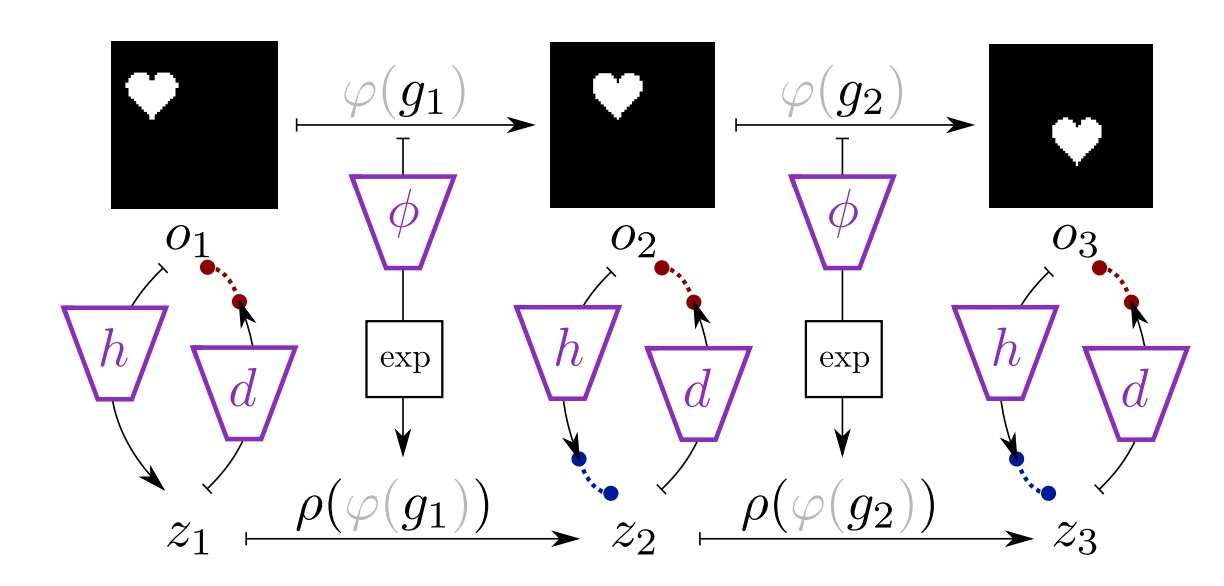
\includegraphics[width=0.75\linewidth]{./hae_arch.jpeg}
  \end{center}
  \caption{The HAE's architecture (figure borrowed from \cite{keurti2023homomorphism})}
  \label{fig:hae_arch}
\end{figure}

Figure \ref{fig:hae_arch} details the architecture of the autoencoder. It consists of three deterministic neural networks:
\begin{itemize}
\item the encoder $h$, that learns representations of the inputs (henceforth called the \textit{observations})
\item the decoder $d$, a decoder for $h$, and
\item the transformation encoder $\phi$, which, if given a transformation in the space of observations, learns an analogous one in the space of latents.
\end{itemize}
The input to the model consists of a trace of observations and actions. The model is trained to minimize a combined prediction-reconstruction loss, the details of which can be found in section \ref{sec:training_loss}.

\subsection{A Walkthrough of the Encoding Process}
 For the purposes of illustration, let us assume that a single transformation has occurred, meaning that the trace is of the form $(o_1, g_1, o_2)$. The latents computed by $h$ for both observations are given as 
 \[ 
   z_1 = h(o_1) \quad z_2 = h(o_2)
 .\]
 The representation of the transformation in latent space is given by \footnote{This is not entirely true. The details of the interaction between $\phi$, $\varphi$, and $\text{exp}$ can be found in appendix \ref{app:lie_groups}.}
 \[ 
   \tilde{g}_1 = \phi(g_1)
 .\]
 
 There are two ``gaps'' in the encoding process that are the targets of minimization:
 \begin{enumerate}
 \item  The \textit{prediction} gap $||z_2 - \tilde{g}_1(z_1)||_2^2$, and
 \item The \textit{reconstruction} gap $||o_2 - d(\tilde{g}_1(z_1))||_2^2$.
 \end{enumerate}

 Clearly, minimizing the prediction gap works to ensure that transformations in the latent space are consistent with transformations in the observation space, and minimizing the reconstruction gap works to ensure that the observation encoder actually learns something meaningful. Minimizing the reconstruction gap also plays the critical role of ensuring that $\phi$ does not end up being the trivial (identity) representation.

 \subsection{Training Loss}
 \label{sec:training_loss}
 For a trace $(o_1, g_1, o_2, g_2, ..., g_{N-1}, o_N)$, the full form of the losses are given by:
 \[ 
 L_{\text{pred}}^N = \sum_{t = 2}^{N+1} ||z_{t} - \bigl ( \prod_{i = 1}^{t-1} \phi(g_i)  \bigr)h(o_1)||_2^2
 ,~\text{and}\]
 \[ 
   L_{\text{rec}}^N = \sum_{t = 2}^{N+1} ||o_t - d\Bigl ( \prod_{i = 1}^{t-1} \phi(g_i)  h(o_1)\Bigr )||_2^2
 .\]

 Let us analyze the prediction loss. For any single term of the summation, $||z_{t} - \bigl ( \prod_{i = 1}^{t-1} \phi(g_i)  \bigr)h(o_1)||$, the minimizer is that $h$ and $\phi$ result in the \textit{cumulative prediction gap} getting minimized. The cumulative minimization gap is the gap between the encoding of the $t^{th}$ observation, and the predicted encoding when we start from the very first latent $z_1$.

 Thus, minimzing the sum is equivalent to ensuring that no matter how many transformations are performed on the observations, we need only take the first encoding, and operate exclusively in latent space, composing the transformations $\phi(g_i)$ to get the encoding of the final observation.

 Similar intuition can be built for the reconstruction loss. It essentially minimizes the same gap that the prediction loss does, but projected back into observation space.

 The combined loss is given by $L_{\text{pred}}^N + \gamma L_{\text{rec}}^N$.
 \subsection{Structural properties of HAE representations}
 \label{sec:structural_properties}
 \textbf{Representations of observations:} The encoder $h: O \rightarrow Z$ learns \textit{group-structured representations} \citep{higgins2018definition} if 
 \begin{itemize}
 \item $Z$ permits the group acting on $O$ to act on itself.
 \item The encoder $h$ is equivariant to the group action, i.e., for all $o \in O$ and $g \in G$, $h(g_Oo) = g_Zh(o)$.
 \end{itemize}
\newpage 
 \textbf{Representations of transformations:} The representation $\phi$ is \textit{disentangled} with respect to some decomposition $(G_1 \times G_2 \times ... \times G_n)$ of $G$ if 
 \begin{itemize}
 \item $Z$ is also decomposable into the same number of units $n$ as $G$ is.
 \item $\phi$ is also decomposable into $n$ units $\phi_1, \phi_2, ..., \phi_n$ (this is enforced through a sparsity regularizer)
 \item Each unit $Z_i$ permits the group $G_i$ to act on it.
 \item The action of $G$ on $Z$ (the form of which is learned by $\phi$) is decomposable as 
   \[ 
   g_Zz = \phi(g_1 \times g_2 \times ... \times g_n)(z_1 \times z_2 \times ... \times z_n) = \phi_1(g_1)z_1 \times \phi_2(g_2)z_2 \times ... \times \phi_n(g_n)z_n
   .\]
   
 \end{itemize}
 There are multiple justifications for why such properties are desirable: that they allow for improved interpretability; that control over representations is easier; that they align better with physics-based real-world transformations. \cite{higgins2018definition} and \cite{higgins2022symmetrybased} give significantly more detailed arguments in favour of these properties than will be presented here.

 
 \subsection{Assumptions about the Data-Generating Process}
 Below, I expand on the assumptions needed for the structure of section \ref{sec:structural_properties} to hold. These assumptions are taken from \cite{keurti2023homomorphism}.

 The process by which the data are generated involves a smooth manifold $W$ of world states, and a vector space $W*$ on which transformations are performed. It is assumed that there is a diffeomorphic map $m: W \rightarrow W*$. The action of $g \in G$ on $W$ is actually taken to be the result of mapping into $W*$, taking the action of $g$ in $W*$, and then mapping the result back into $W$:
 \[ 
 g_Ww \triangleq m^{-1}(g_{W*}m(w))
 ~\text{where}~w \in W\]

 The world states are mapped to observations by a diffeomorphic map $b: W \rightarrow O$, and actions of a group on the observation space can actually be arrived at through actions of the group on $W*$. Figure \ref{fig:diffhae} should help build intuition about the relationship between the different sets.

 \begin{figure}[h]
 \begin{center}
   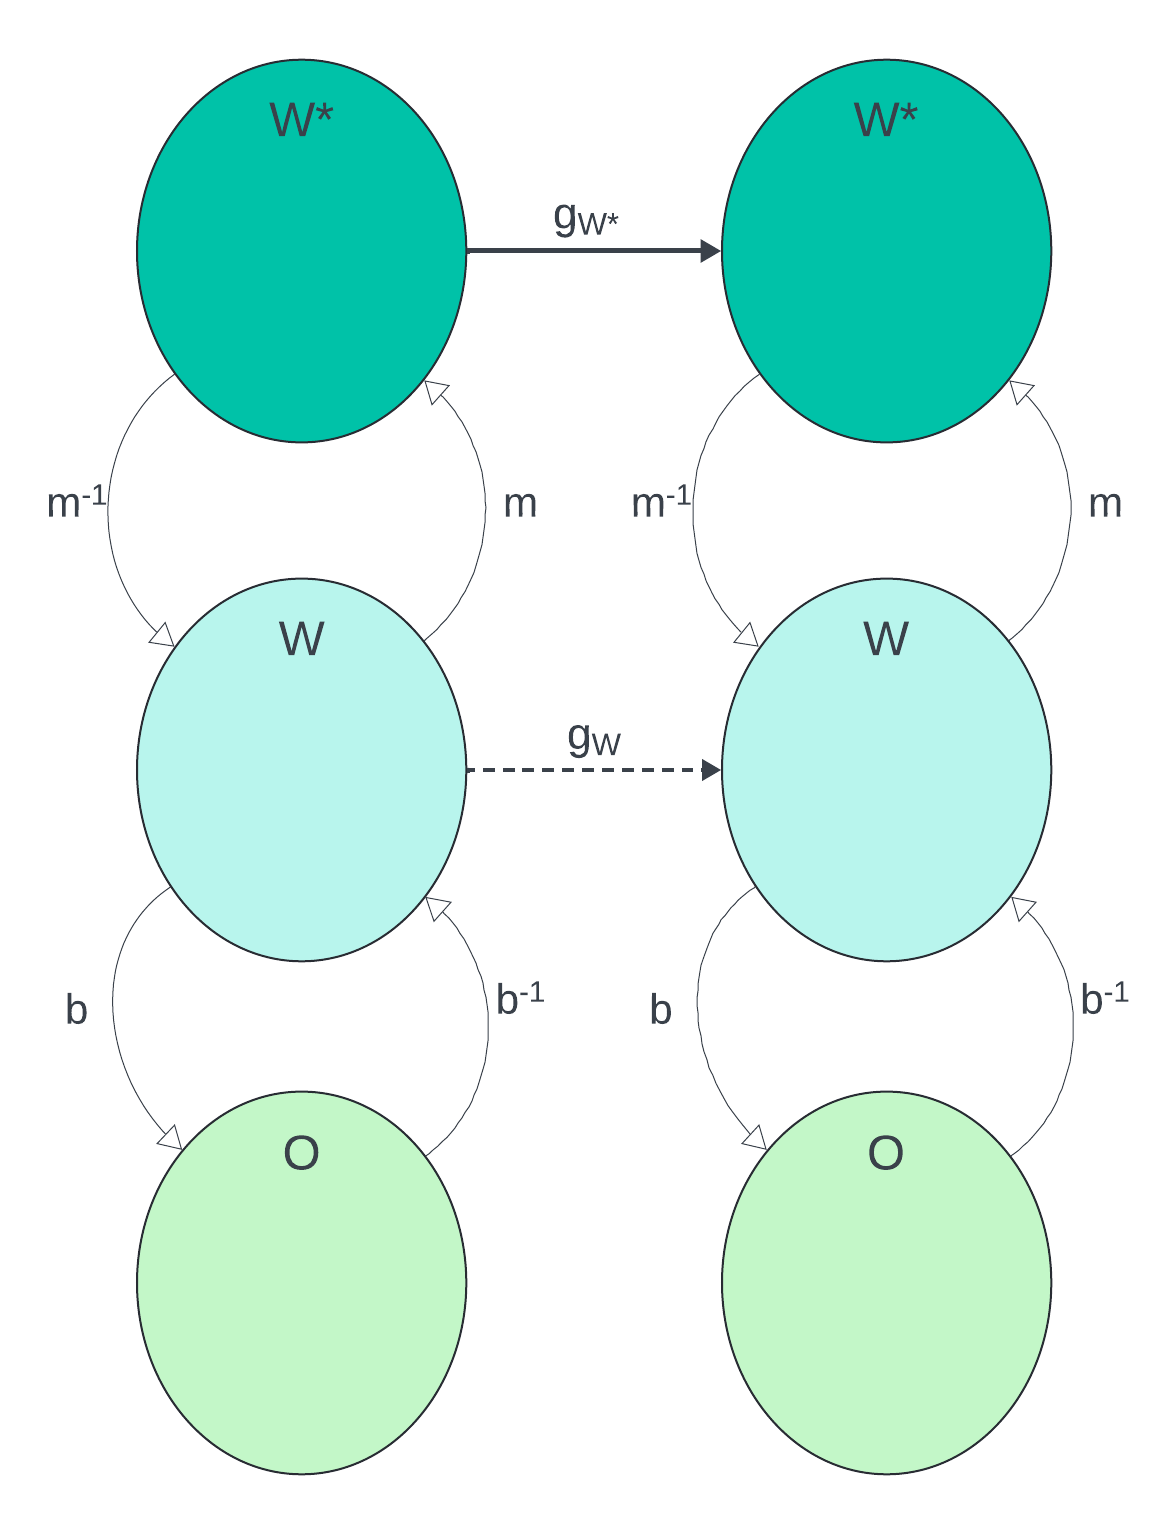
\includegraphics[width=0.5\linewidth]{./DiffHAE.png}
 \end{center} 
 \caption{An illustration of the sets and spaces involved in the data-generating process}
 \label{fig:diffhae}
\end{figure} 

If these assumptions are adhered to, then the properties of section \ref{sec:structural_properties} hold, in accordance with proposition 1 of \cite{keurti2023homomorphism}.

Thus, we arrive at the main idea behind this report: 
\subsection{Central Motivation}
\label{sec:central_motivation}
\textit{If, given a set of transformations $G$, we can construct set $W$, space $W*$, mappings $m$ and $b$, and represent the transformations as elements of some matrix group $G_{W*}$ acting on $W*$, then we have that the HAE-representations for the set $G$ are symmetry-based and disentangled.}

\section{The Diffusion Process}
I have selected \textit{diffusion}, as detailed in \cite{sohldickstein2015deep}, as the set of transformations for which the constructions of \ref{sec:central_motivation} will be attempted. The motivations behind this are simple:
\begin{itemize}
\item The diffusion process, at a first glance, fits the framework of iterative observations and transformations that the HAE is designed for.
\item Symmetry-based and disentangled representations of the diffusion process could potentially be interpretable, and at the very least provide control during generation.
\item The learned representations of the denoising process might have performance benefits, since the HAE is designed to learn representations that are useful for prediction and reconstruction.
\item The learned representations could be interesting in their own right, potentially shedding light on notions of geometry and symmetry in the diffusion process, similar to the results of \cite{keurti2023homomorphism}.
\end{itemize}

While most of these benefits can only be verified through empirical study, showing that the constructions are possible is the first step, indicating that experimentation is warranted. I will now detail the requisite constructions.
\subsection{The Set $W$}
Since our observation space is pixel space, i.e. the set of all $n \times n$ matrices, I construct $W$ to be the space $R^{n^2}$, with $b^{-1}$  being the linearization operation, and $b$ the reconstruction operation. It is required to prove that $b$ is a \textit{diffeomorphism}, which can be done by proving the following:
\begin{itemize}
\item $W$ and $O$ are smooth manifolds.
\item There exist projections from both $W$ and $O$ onto some finite-dimensional vector space, such that the map between these projections that is equivalent to $b$ is smooth, invertible, and whose inverse is smooth.
\end{itemize}

From example 1.24 of \cite{lee2013introduction}, we have that since both $W$ and $O$ are smooth manifolds, since they are both finite-dimensional vector spaces.
If we take the projection from $W$ onto $\mathbb{R}^{n^2}$ to be the linearization (which is the same as taking $\psi = b$), and taking the projection from $O$ onto $\mathbb{R}^{n^2}$ to be the identity, then the map between these projections is the identity, which is smooth, invertible, and whose inverse is smooth. Thus, $b$ is a diffeomorphism.

\subsection{The Space $W*$}
I construct $W*$ to be the space $\mathbb{R}^{n^2 + 1}$. The map $m: \mathbb{R}^{n^2} \rightarrow \mathbb{R}^{n^2 + 1}$ is defined as 
\[ 
  m([v_1, v_2, ..., v_{n^2}]^T) = [v_1, v_2, ..., v_{n^2}, 1]^T
\]
Note that $m$ is not a surjection, and thus can only be a bijection if we restrict $W*$ to the image of $W$ under $m$. This would, however, remove its status as a vector space. Therefore, we must accept the slightly weakened construction of $W* = \text{Im}_m(W) + \mathbf{0}_{n^2 + 1}$. Since in practice, we will never encounter the vector $\mathbf{0}_{n^2 + 1}$, it is of practical relevance to proceed with $m^{-1}:\text{Im}_m(W) \rightarrow W$ as the inverse we would have gotten otherwise:
\[ 
  m^{-1}([v_1, v_2, ..., v_{n^2}, 1]^T) = [v_1, v_2, ..., v_{n^2}]^T
.\]

From similar reasoning as in the previous section, $m$ is a diffeomorphism. (Here, the finite-dimensional vector space that both $W$ and $W*$ are mapped onto is $\mathbb{R}^{n^2}$)

\subsection{The Matrix Group $G_{W*}$}

In order to represent the denoising operation as arising from a matrix multiplication (and therefore as the result of a group's action on a set), we must first relate the structure of the denoising process to that of the noising process. This is due to the fact that the noising process, being pre-determined and Gaussian, can be written down as 
\[ 
x_{k+1} = x_k + \sigma \epsilon ~\text{where}~\epsilon \sim \mathcal{N}(0, I)
.\]

If the $x_i$'s belong to $\mathbb{R}^n$, then the above operation can be represented as a matrix multiplication in $\mathbb{R}^{n+1}$:
\[ 
  x_{k+1} = \left(
  \begin{bmatrix}
    1 & 0 & 0 & ... & 0 & \sigma \epsilon_1 \\
    0 & 1 & 0 & ... & 0 & \sigma \epsilon_2 \\
    0 & 0 & 1 & ... & 0 & \sigma \epsilon_3 \\
    \vdots & \vdots & \vdots & \ddots & \vdots & \vdots \\
    0 & 0 & 0 & ... & 1 & \sigma \epsilon_n \\ 
    0 & 0 & 0 & ... & 0 & 1
  \end{bmatrix}
\begin{bmatrix}
  x_{k,1} \\
  x_{k,2} \\ 
  x_{k,3} \\ 
  \vdots \\ 
  x_{k,n} \\
  1
  \end{bmatrix} 
\right)_{[1:n]}
.\]

Thus, if a similar update equation can be arrived at for the denoising process, then we can represent it too as a matrix-multiplication.

To do so, I refer to equation 58 of \cite{luo2022understanding}, which offers a lower-bound on the ELBO:
\[ 
  \log p(x) \geq \underbrace{\mathbb{E}_q(x_1 | x_0)[\log p_\theta(x_0 | x_1)]}_{\text{reconstruction term}} - \underbrace{D_{KL}(q(x_T|x_0)||p(x_T))}_{\text{prior matching term}} - \sum_{t = 2 }^{T } \mathbb{E}_q(x_t | x_0 ) \underbrace{[D_{KL}(q(x_{t-1}|x_t, x_0)|| p_\theta(x_{t-1}|x_t))]}_{\text{denoising matching term}}
.\]

The \textit{denoising matching term} tells us that it makes sense to have the learned denoiser $p_\theta(x_{t-1}|x_t)$ be as close as possible to the ground-truth denoiser $q(x_t | x_{t-1}, x_0)$.

From equation 84 of \cite{luo2022understanding}, we have that the denoising process is distributed as 
\[ 
  q(x_t | x_{t-1}, x_0) \propto \mathcal{N}(\underbrace{\frac{\sqrt{\alpha_t}(1 - \bar \alpha_{t-1})x_t + \sqrt{\bar \alpha_{t-1}}(1 - \alpha_t)x_0}{1 - \bar \alpha_t}}_{\mu_q(x_t, x_0)}, \underbrace{\frac{(1 - \alpha_t)(1 - \bar \alpha_{t-1})}{1 - \bar \alpha_t}I}_{\Sigma_q(t)})
.\]

Thus, we have that the ground-truth denoising process is also normally distributed, meaning that the learned one can be parameterized as $\mathcal{N}(\mu_\theta(x_t),\Sigma(t))$, with the mean being the output of a neural network, seeing as we do not have access to the ground-truth image $x_0$.

Thus, the denoising update rule for a learned denoising process $p_\theta$ can be written as 
\[ 
  x_{t-1} = \mu_\theta(x_t) + \Sigma(t) \epsilon ~\text{where}~\epsilon \sim \mathcal{N}(0, I)
,\]

which can, in turn, be represented as a matrix multiplication in $\mathbb{R}^{n+1}$:
\[ 
\begin{bmatrix}
  x_{t-1,1} \\ 
  x_{t-1,2} \\ 
  x_{t-1,3} \\ 
  \vdots \\ 
  x_{t-1,n} \\ 
  1 
\end{bmatrix} = 
\begin{bmatrix}
  \frac{\mu_\theta(x_t)_1}{x_{t, 1}} & 0 & 0 & ... & 0 & \Sigma(t)\epsilon_1 \\
  0 & \frac{\mu_\theta(x_t)_2}{x_{t, 2}} & 0 & ... & 0 & \Sigma(t)\epsilon_2 \\ 
  0 & 0 & \frac{\mu_\theta(x_t)_3}{x_{t, 3}} & ... & 0 & \Sigma(t)\epsilon_3 \\ 
  \vdots & \vdots & \vdots & \ddots & \vdots & \vdots \\ 
  0 & 0 & 0 & ... & \frac{\mu_\theta(x_t)_n}{x_{t, n}} & \Sigma(t)\epsilon_n \\ 
  0 & 0 & 0 & ... & 0 & 1 
  \end{bmatrix}
\begin{bmatrix}
  x_{t,1} \\ 
  x_{t,2} \\ 
  x_{t,3} \\ 
  \vdots \\ 
  x_{t,n} \\ 
  1
\end{bmatrix}
.\]

Thus, we have that denoising can be represented as a matrix-multiplication. To ensure that the set that these matrices come from is a (compact) group, we just set it to be the subset of $GL(n^2 + 1, \mathbb{R})$ whose elements' absolute values do not exceed a constant $C \sim 1$ (assuming the dynamic range of images is between 0 and 1). Compactness here arises from the fact that both $x_{t, i}$ and $\mu_\theta(x_t)_i$ represent pixel values, and this means that each element is bounded.\footnote{I am not certain of the exact form of the bound, but it clearly depends on $\Sigma(t)$, and therefore on the step-size scheme ${\alpha_t}$.}.



\section{Weaknesses}
The main weakness of this approach appears to be that the final column of the matrix group is always the result of a stochastic process. While we could simply hand-wave away the stochasticity by attributing it to the randomness of sampling from the set of all possible transformations, the fact that the individual elements are Gaussian suggests that something more concrete can be said about this form of the diffusion group. 

An intuitive direction of inquiry is to see if any of my assertions can be said to hold in expectation. While this is trivial over a single step (since the last column would all get clipped down to zero, leaving us with a linear transformation), the fact that the mean changes at every step means that the distribution over the entire denoising process is significantly more complex.



\bibliographystyle{tmlr}
\bibliography{tmlr.bib}

\appendix
\section{Appendix}

 \subsection{A Note on Lie Algebras and Lie Groups}
 \label{app:lie_groups}
 If we are to work with groups, then there is not necessarily any restriction on what form the group's elements can take. They need only satisfy the group axioms, which means that any set of arbitrarily complex structures that is composable, closed under composition,  and contains an identity and inverses, can be used to represent the set of transformations we are interested in. If, however, the set of transformations can be represented as elements of a smooth manifold, then there are certain simplifications that can be made.

 A group that is also a smooth manifold is termed a \textit{Lie group}. These manifolds are not necessarily vector spaces, since while they might belong to some subset $E \in \mathbb{R}^n$, we do not require that $\mathbf{0} \in E$. It is helpful to think of them as subsets that are offset from the origin by some amount.

 Given some Lie group $G$, the tangent space of this manifold around the identity element forms its \textit{Lie algebra} $\mathfrak{g}$. The Lie algebra has the benefit of being a vector space. We cannot immediately use the algebra to represent the group, however, since it is a linear approximation of the group at a point, and thus incurs some error.

 Before we begin to tackle this error, we must first understand the notion of the \textit{representation} of a group on a set. Intuitively, the group's representation on a set is the form that the elements of the group take to be able to act on the set. For a concrete example, consider the group $G$ of invertible linear transformations. Without specifying exactly what space/set is being transformed, the group remains as an abstract concept. If, however, we specify that we are working with $\mathbb{R}^n$, we can say that the representation of $G$ on this space is the set of invertible $n \times n$ matrices, which just so happens to have the notation $GL(n, \mathbb{R})$.

 Since we are working with concrete, real vector spaces, it helps to speak of groups in terms of their representations on these spaces. From now on, let us treat the representation of any group on the vector space we are working on as the group itself, and call it the \textit{matrix} group for that space.
 
 From definiton 2.2 of \cite{hall2000elementary}, we have that any \textit{closed subgroup} of $GL(n, \mathbb{R})$ is a Lie group. Corollary 3.44 of \cite{hall2015lie} tells us that if our lie group is \textit{compact}, then there is a bijective map between the group and its lie algebra.

 This bijective map is given by $\text{exp}: \mathfrak{g} \rightarrow G$, defined as 
 \[ 
 e^X = \sum_{m = 0 }^{\infty} \frac{X^m }{m!}
 \]
 From definition 2.4 of \cite{hall2015lie}, a matrix group is compact if $\exists C \in \mathbb{R}$ such that for all $A \in G$, $|A_{ij}| \leq C$ for all $1 \leq i, j \leq n$.

 From proposition 2.1 of \cite{hall2015lie}, the matrix exponential converges for all square $X$. 


 Thus, in summary, we have that if we are working with a compact matrix group, we can instead work with its lie algebra, with the knowledge that the two are equivalent. This realization manifests in the HAE through the fact that $\phi$ actually takes elements of the lie algebra as input.

 Let the matrix group acting on observation space be denoted by $G$, with a lie algebra of $\mathfrak{g}$, and the matrix group acting on the latent space be denoted by $\tilde{G}$, with a lie algebra of $\tilde{\mathfrak{g}}$. Then $\phi$ learns to map between $\mathfrak{g}$ and $\tilde{\mathfrak{g}}$, after which the exponential map $\text{exp}:\tilde{\mathfrak{g}}\rightarrow \tilde{G}$ is used to get a valid matrix transformation for the latent space.
 
\subsection{A Note on Diffeomorphisms}
A central idea for proving smoothness is the notion of a \textit{coordinate chart}. A coordinate chart (or just a chart) on a manifold $M$ is a pair $(U, \phi)$, where $U$ is an open subset of $M$, and $\phi: U \rightarrow \mathbb{R}^n$ is a homeomorphism. The homeomorphism property is what allows us to map between the manifold and $\mathbb{R}^n$.
In order to prove that a function $f$ between two manifolds $M$ and $N$ is smooth, we need to show that for point $p \in M$, we can find charts $(U, \phi)$ and $(V, \psi)$ such that $p \in U$, $f(p) \in V $, and the function $f$, written as $\psi \circ f \circ \phi^{-1}$, is a smooth function between $\mathbb{R}^n$ and $\mathbb{R}^n$.

For a more complete treatment of the smooth manifolds, see \cite{lee2013introduction}.

\end{document}
